%
% einleitung.tex -- Beispiel-File für die Einleitung
%
% (c) 2020 Prof Dr Andreas Müller, Hochschule Rapperswil
%
\section{Einleitung\label{kreismembran:section:teil0}}
\rhead{Membran}
Eine Membran oder selten ein Schwingblatt ist laut Duden \cite{kreismembran:Duden:Membran} ein ``dünnes Blättchen aus Metall, Papier o. Ä., das durch seine Schwingungsfähigkeit geeignet ist, Schallwellen zu übertragen \dots''. 
Ein dünnes Blättchen aus Metall zeig jedoch nicht die selben dynamischen Eigenschaften wie ein gespanntes Stück Papier. 
Beschreibt man das dynamische Verhalten, muss zwischen einer dünnen Platte und einer Membran unterschieden werden \cite{kreismembran:membrane_vs_thin_plate}. 
Eine dünne Platte zum Beispiel aus Metall, wirkt selbst entgegen ihrer Deformation, sobald sie gekrümmt wird. 
Eine Membran auf der anderen Seite besteht aus einem Material, welches sich ohne Kraftaufwand verbiegen lässt, wie zum Beispiel Papier. 
Bevor Papier als schwingende Membran betrachtet werden kann, wird jedoch noch eine Spannung $ T $ benötigt, welche das Material daran hindert, aus der Ruhelage gebracht zu werden. 

Ein geläufiges Beispiel einer Kreismembran ist eine runde Trommel. 
Sie besteht herkömmlicherweise aus einem Leder (Fell), welches auf einen offenen Zylinder (Zargen) aufgespannt wird. 
Das Leder alleine erzeugt nach einem Aufschlag keine hörbaren Schwingungen. 
Sobald das Fell jedoch über den Zargen gespannt wird, kann das Fell auf verschiedensten Weisen weiter schwingen, was für den Klang der Trommel verantwortlich ist. 
Wie genau diese Schwingungen untersucht werden können, wird in der folgenden Arbeit diskutiert.
	

\subsection{Annahmen} \label{kreimembran:annahmen}
Um die Wellengleichung herzuleiten \cite{kreismembran:wellengleichung_herleitung}, muss ein Modell einer Membran definiert werden. 
Das untersuchte Modell erfüllt folgende Eigenschaften:
\begin{enumerate}[i)]
	\item Die Membran ist homogen. 
	Dies bedeutet, dass die Membran über die ganze Fläche die selbe Dichte $ \rho $  und Elastizität hat. 
	Durch die konstante Elastizität ist die ganze Membran unter gleichmässiger Spannung $ T $.
	\item Die Membran ist perfekt flexibel. 
	Damit ist gemeint, dass die Membran ohne Kraftaufwand verbogen werden kann. 
	Die Membran ist dadurch nicht allein stehend schwingfähig, hierzu muss sie mit einer Kraft $ T $ gespannt werden.
	\item Die Membran kann sich nur in Richtung ihrer Normalen in kleinem Ausmass auslenken.
	Auslenkungen in der Ebene der Membran sind nicht möglich.
	\item Die Membran erfährt keine Art von Dämpfung. 
	Die Membran wird also nicht durch ihr umliegendes Medium abgebremst noch erfährt sie Reibungsverluste durch Deformation.
	
\end{enumerate}

\subsection{Wellengleichung} Um die Wellengleichung einer Membran herzuleiten, wird vorerst eine schwingende Saite betrachtet.
Es lohnt sich, das Verhalten einer Saite zu beschreiben, da eine Saite dasselbe Verhalten wie eine Membran aufweist, mit dem Unterschied einer fehlenden Dimension.
Die Verbindung zwischen Membran und Saite ist intuitiv ersichtlich, stellt man sich einen Querschnitt einer Trommel vor.
\begin{figure}
	
	\begin{center}		
		% 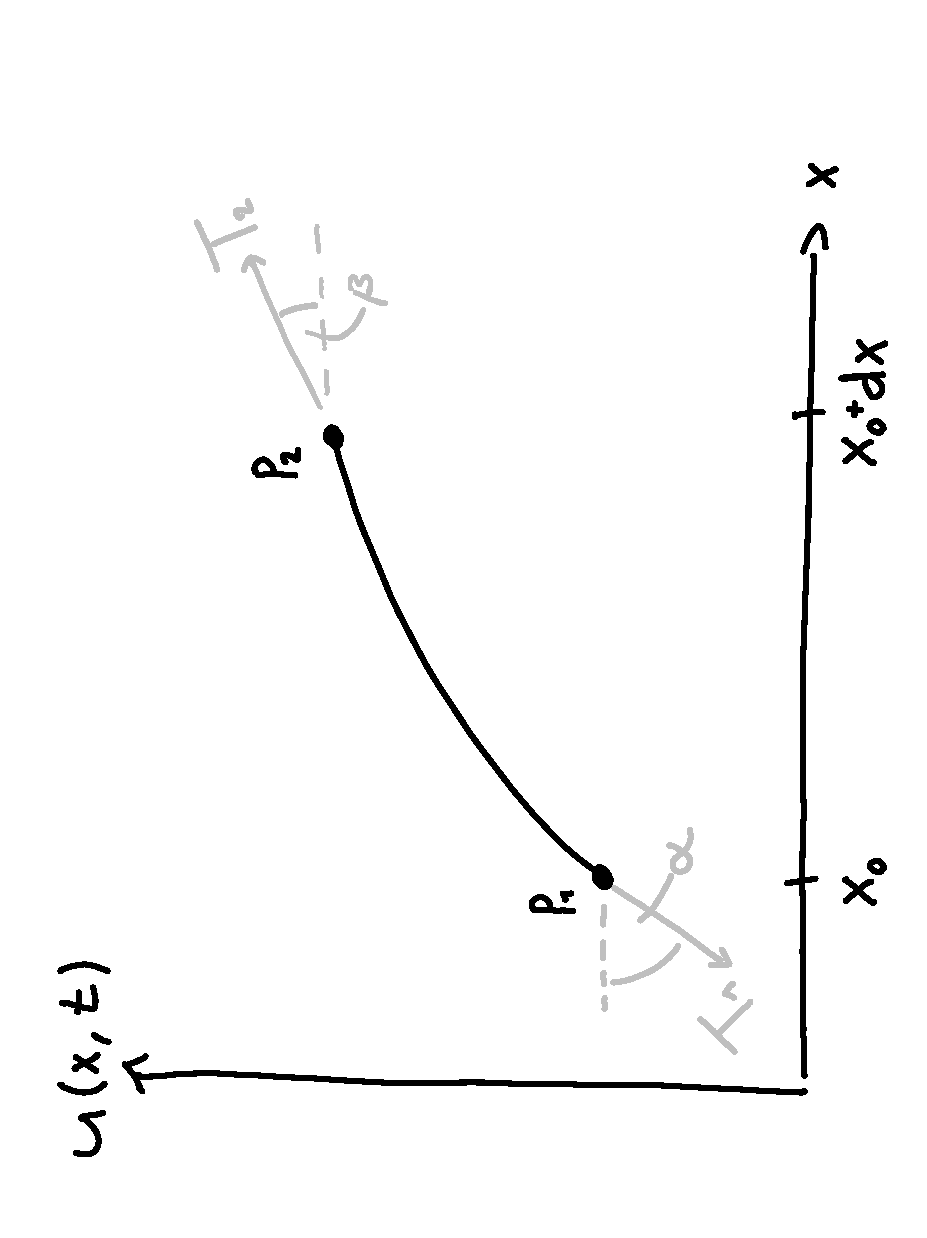
\includegraphics[width=5cm,angle=-90]{papers/kreismembran/images/Saite.pdf}
		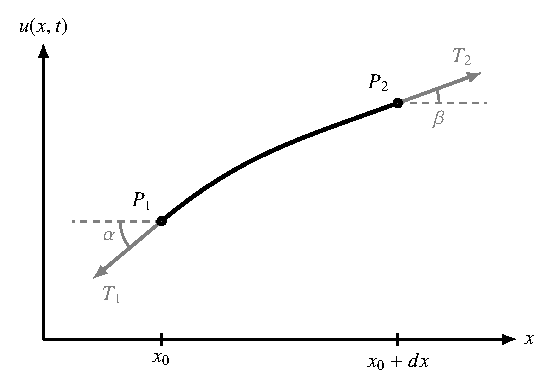
\includegraphics[]{papers/kreismembran/images/TikzSaite.pdf}
		\caption{Infinitesimales Stück einer Saite}
		\label{kreismembran:im:Saite}
	\end{center}	
\end{figure}

In Abbildung \ref{kreismembran:im:Saite} ist ein infinitesimales Stück einer Saite mit Länge $ dx $ skizziert.
Wie für die Membran ist die Annahme iii) gültig, es entsteht keine Bewegung entlang der $ x $-Achse.
Um dies zu erfüllen, muss der Punkt $ P_1 $ gleich stark entgegen der $ x $-Achse gezogen werden wie der Punkt $ P_2 $ in Richtung der $ x $-Achse gezogen wird. 
Ist $ T_1 $ die Kraft, welche mit Winkel $ \alpha $ auf Punkt $ P_1 $ wirkt sowie $ T_2 $ und $ \beta$ das analoge für Punkt $ P_2 $ ist, so können die Kräfte 
\begin{equation}\label{kreismembran:eq:no_translation}
	T_1 \cos \alpha = T_2 \cos \beta = T
\end{equation}
gleichgesetzt werden. 
Das dynamische Verhalten der senkrechten Auslenkung $ u(x,t) $ muss das newtonsche Gesetz 
\begin{equation*}
	\sum F = m \cdot a
\end{equation*} 
befolgen. Die senkrecht wirkenden Kräfte werden mit $ T_1 $ und $ T_2 $ ausgedrückt, die Masse als Funktion der Dichte $ \rho $ und die Beschleunigung in Form der zweiten Ableitung als
\begin{equation*}
	T_2 \sin \beta - T_1 \sin \alpha = \rho dx \frac{\partial^2 u}{\partial t^2} .
\end{equation*}
Die Gleichung wird durch $ T $ dividiert, wobei $ T $ nach \eqref{kreismembran:eq:no_translation} geschickt gewählt wird. Somit kann
\begin{equation*}
	\frac{T_2 \sin \beta}{T_2 \cos \beta} - \frac{T_1 \sin \alpha}{T_1 \cos \alpha} = \frac{\rho dx}{T} \frac{\partial^2 u}{\partial t^2}
\end{equation*}
vereinfacht als  
\begin{equation*}
	\tan \beta - \tan \alpha = \frac{\rho dx}{T} \frac{\partial^2 u}{\partial t^2}
\end{equation*}
geschrieben werden. 
Der $ \tan \alpha $ entspricht der örtlichen Ableitung von $ u(x,t) $ an der Stelle $ x_0 $ und analog der $ \tan \beta $ für die Stelle $ x_0 + dx $.
Die Gleichung wird dadurch zu
\begin{equation*}
	\frac{\partial u}{\partial x} \bigg|_{x_0 + dx} - \frac{\partial u}{\partial x} \bigg|_{x_0} = \frac{\rho dx}{T} \frac{\partial^2 u}{\partial t^2}.
\end{equation*} 
Durch die Division mit $ dx $ entsteht 
\begin{equation*}
	\frac{1}{dx} \left[\frac{\partial u}{\partial x} \bigg|_{x_0 + dx} - \frac{\partial u}{\partial x} \bigg|_{x_0}\right] = \frac{\rho}{T}\frac{\partial^2 u}{\partial t^2}.
\end{equation*}
Auf der linken Seite der Gleichung wird die Differenz der Steigungen durch die Intervalllänge geteilt.
Wenn $ dx $ als unendlich kleines Stück betrachtet wird, ergibt sich als Grenzwert die zweite Ableitung von $ u(x,t) $ nach $ x $. 
Der Term $ \frac{\rho}{T} $ wird durch $ c^2 $ ersetzt, da der Bruch für eine gegebene Membran eine positive Konstante sein muss. 
Damit resultiert die in der Literatur gebräuchliche Form 
\begin{equation}
	\label{kreismembran:Ausgang_DGL}
	\frac{1}{c^2}\frac{\partial^2u}{\partial t^2} = \Delta u.
\end{equation}
In dieser Form ist die Gleichung auch gültig für eine Membran. 
Für den Fall einer Membran muss lediglich der Laplace-Operator $\Delta$ in zwei Dimensionen verwendet werden.